
\paragraph{预测误差与可复核对照}
用MAE和RMSE分别衡量平均绝对偏差及较大误差：
\begin{equation}
 \mathrm{MAE}=N^{-1}\sum_i|y_i-\widehat y_i|,
 \quad \mathrm{RMSE}=\sqrt{N^{-1}\sum_i(y_i-\widehat y_i)^2}.
\end{equation}
\begin{table}[H]\centering\small
\caption{冻结预测器与朴素候选的误差核验；开发期为1月15--31日，正式期为2--12月}
\label{tab:revision-forecast}
\begin{tabular}{llrrrr}\toprule
对象 & 预测方法 & 开发 MAE & 开发 RMSE & 正式 MAE & 正式 RMSE\\\midrule
负荷（kW） & 前一日 & 658.48 & 1148.64 & 650.02 & 1128.39 \\
负荷（kW） & 前一周（选定） & 142.55 & 177.25 & 176.80 & 244.29 \\
负荷（kW） & 近七日均值 & 781.87 & 961.04 & 781.21 & 955.92 \\
负荷（kW） & 周趋势 & 248.25 & 310.44 & 297.49 & 390.92 \\
光伏（kW） & 前一日 & 119.48 & 261.96 & 185.35 & 375.17 \\
光伏（kW） & 前一周 & 137.16 & 280.30 & 214.69 & 419.95 \\
光伏（kW） & 近七日均值（选定） & 96.18 & 203.87 & 153.40 & 303.86 \\
光伏（kW） & 周趋势 & 186.87 & 402.53 & 338.36 & 681.30 \\
电价（元/kWh） & 前一日 & 0.08576 & 0.12877 & 0.08433 & 0.12384 \\
电价（元/kWh） & 前一周（选定） & 0.03829 & 0.04878 & 0.04715 & 0.06535 \\
电价（元/kWh） & 近七日均值 & 0.08160 & 0.10473 & 0.08267 & 0.10527 \\
电价（元/kWh） & 周趋势 & 0.06447 & 0.08176 & 0.07920 & 0.10519 \\
\bottomrule\end{tabular}\end{table}

表中正式期是冻结预测族后的逐日评价，不用其误差重新选型；开发期分数属于回顾性选择窗口。按四个合法发布点分别评估随后六小时，历史修正与官方预报下的净需求MAE分别为264.29和207.41 kW。预测族较简单是模型局限；完美信息费用差同时含交易与控制差异，不能单独用来诊断预测器。
\begin{figure}[H]\centering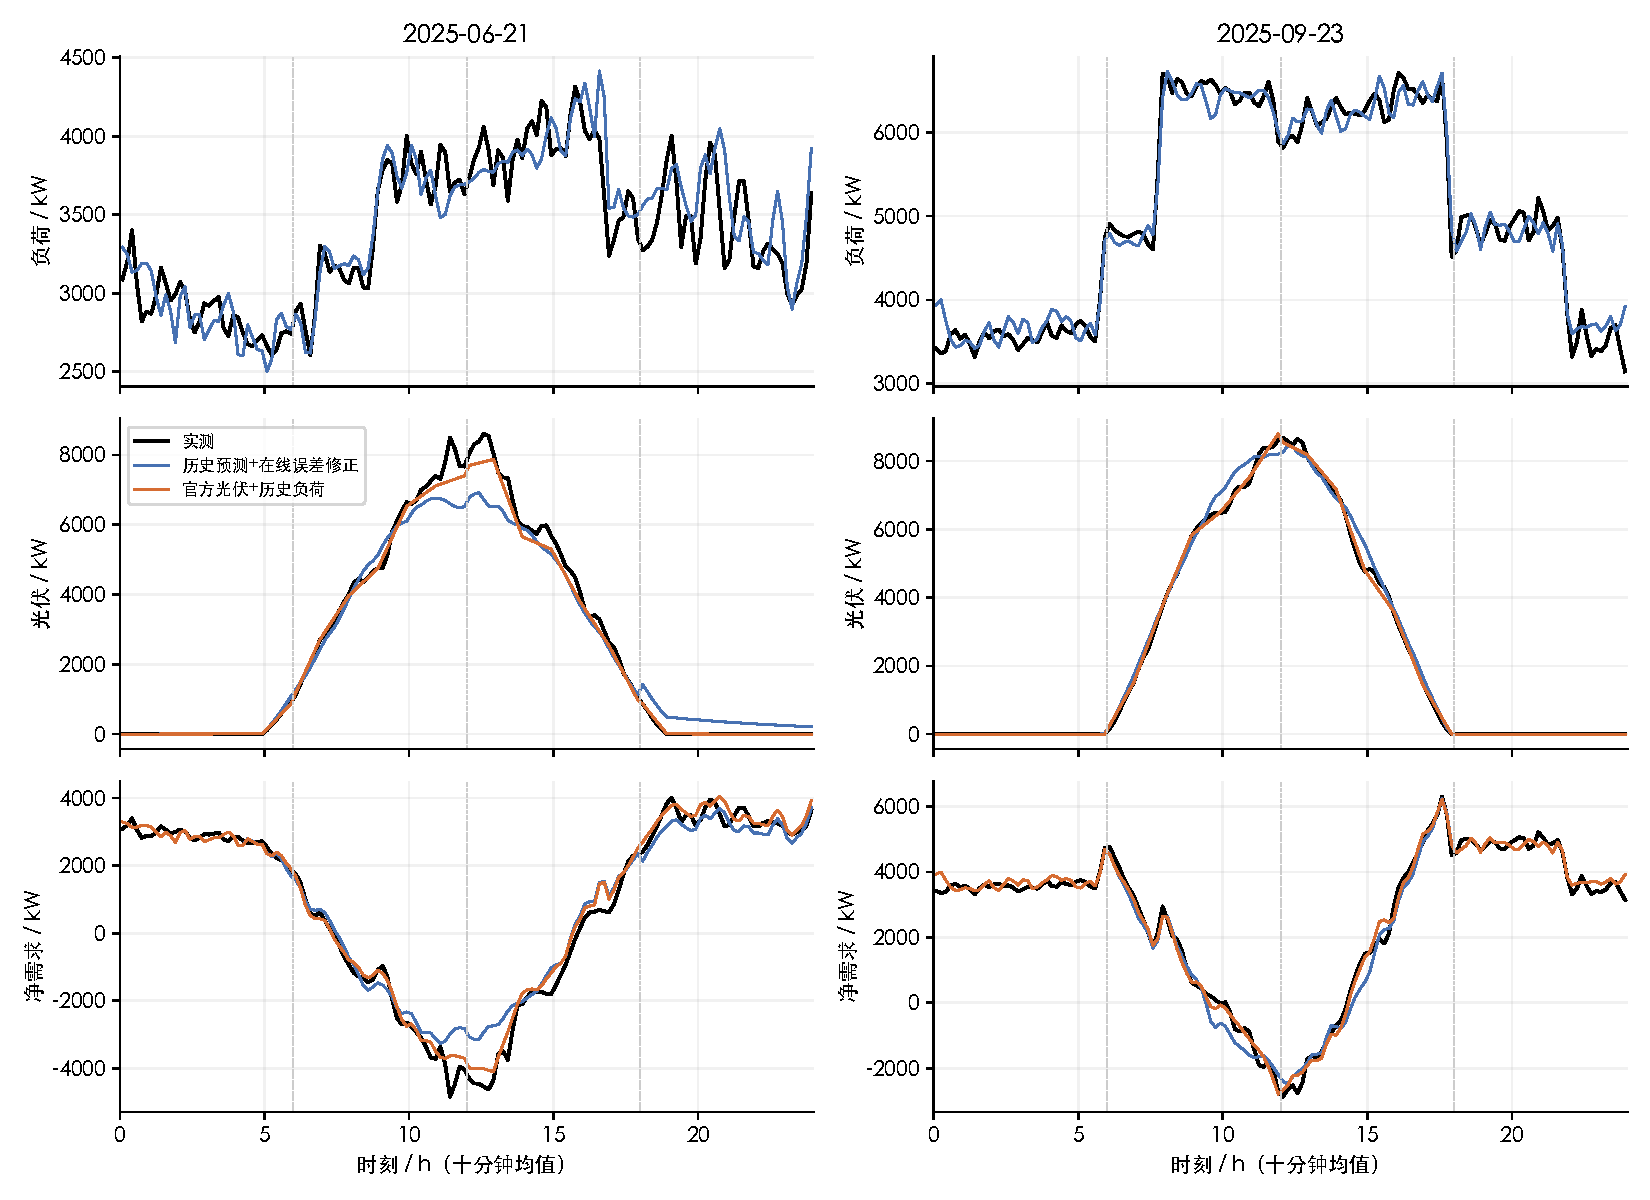
\includegraphics[width=.95\linewidth]{revision/prediction-control/forecast-vs-actual.pdf}\caption{冻结预测与实际轨迹对照；图中各预报遵循其发布时刻}\end{figure}
